\subsection{Electromagnetic Calorimeter (EC) and Pre-Shower Calorimeter (PCAL)}

\subsubsection{Geometry}

Both the EC and PCAL (referred to together as ECAL) calorimeter geometry is implemented through the java geometry service.
The service provides the Geant4 definitions that are read by the GEMC perl API to build the geometry database.

All scintillators are Geant4 volumes. The paddles are assigned the scintillator material and associated with the ECAL hit process routine.
Each scintillator is a trapezoid embedded in a trapezoid mother volume made of air (\F{ecGeometry}).

\begin{figure}
	\centering
	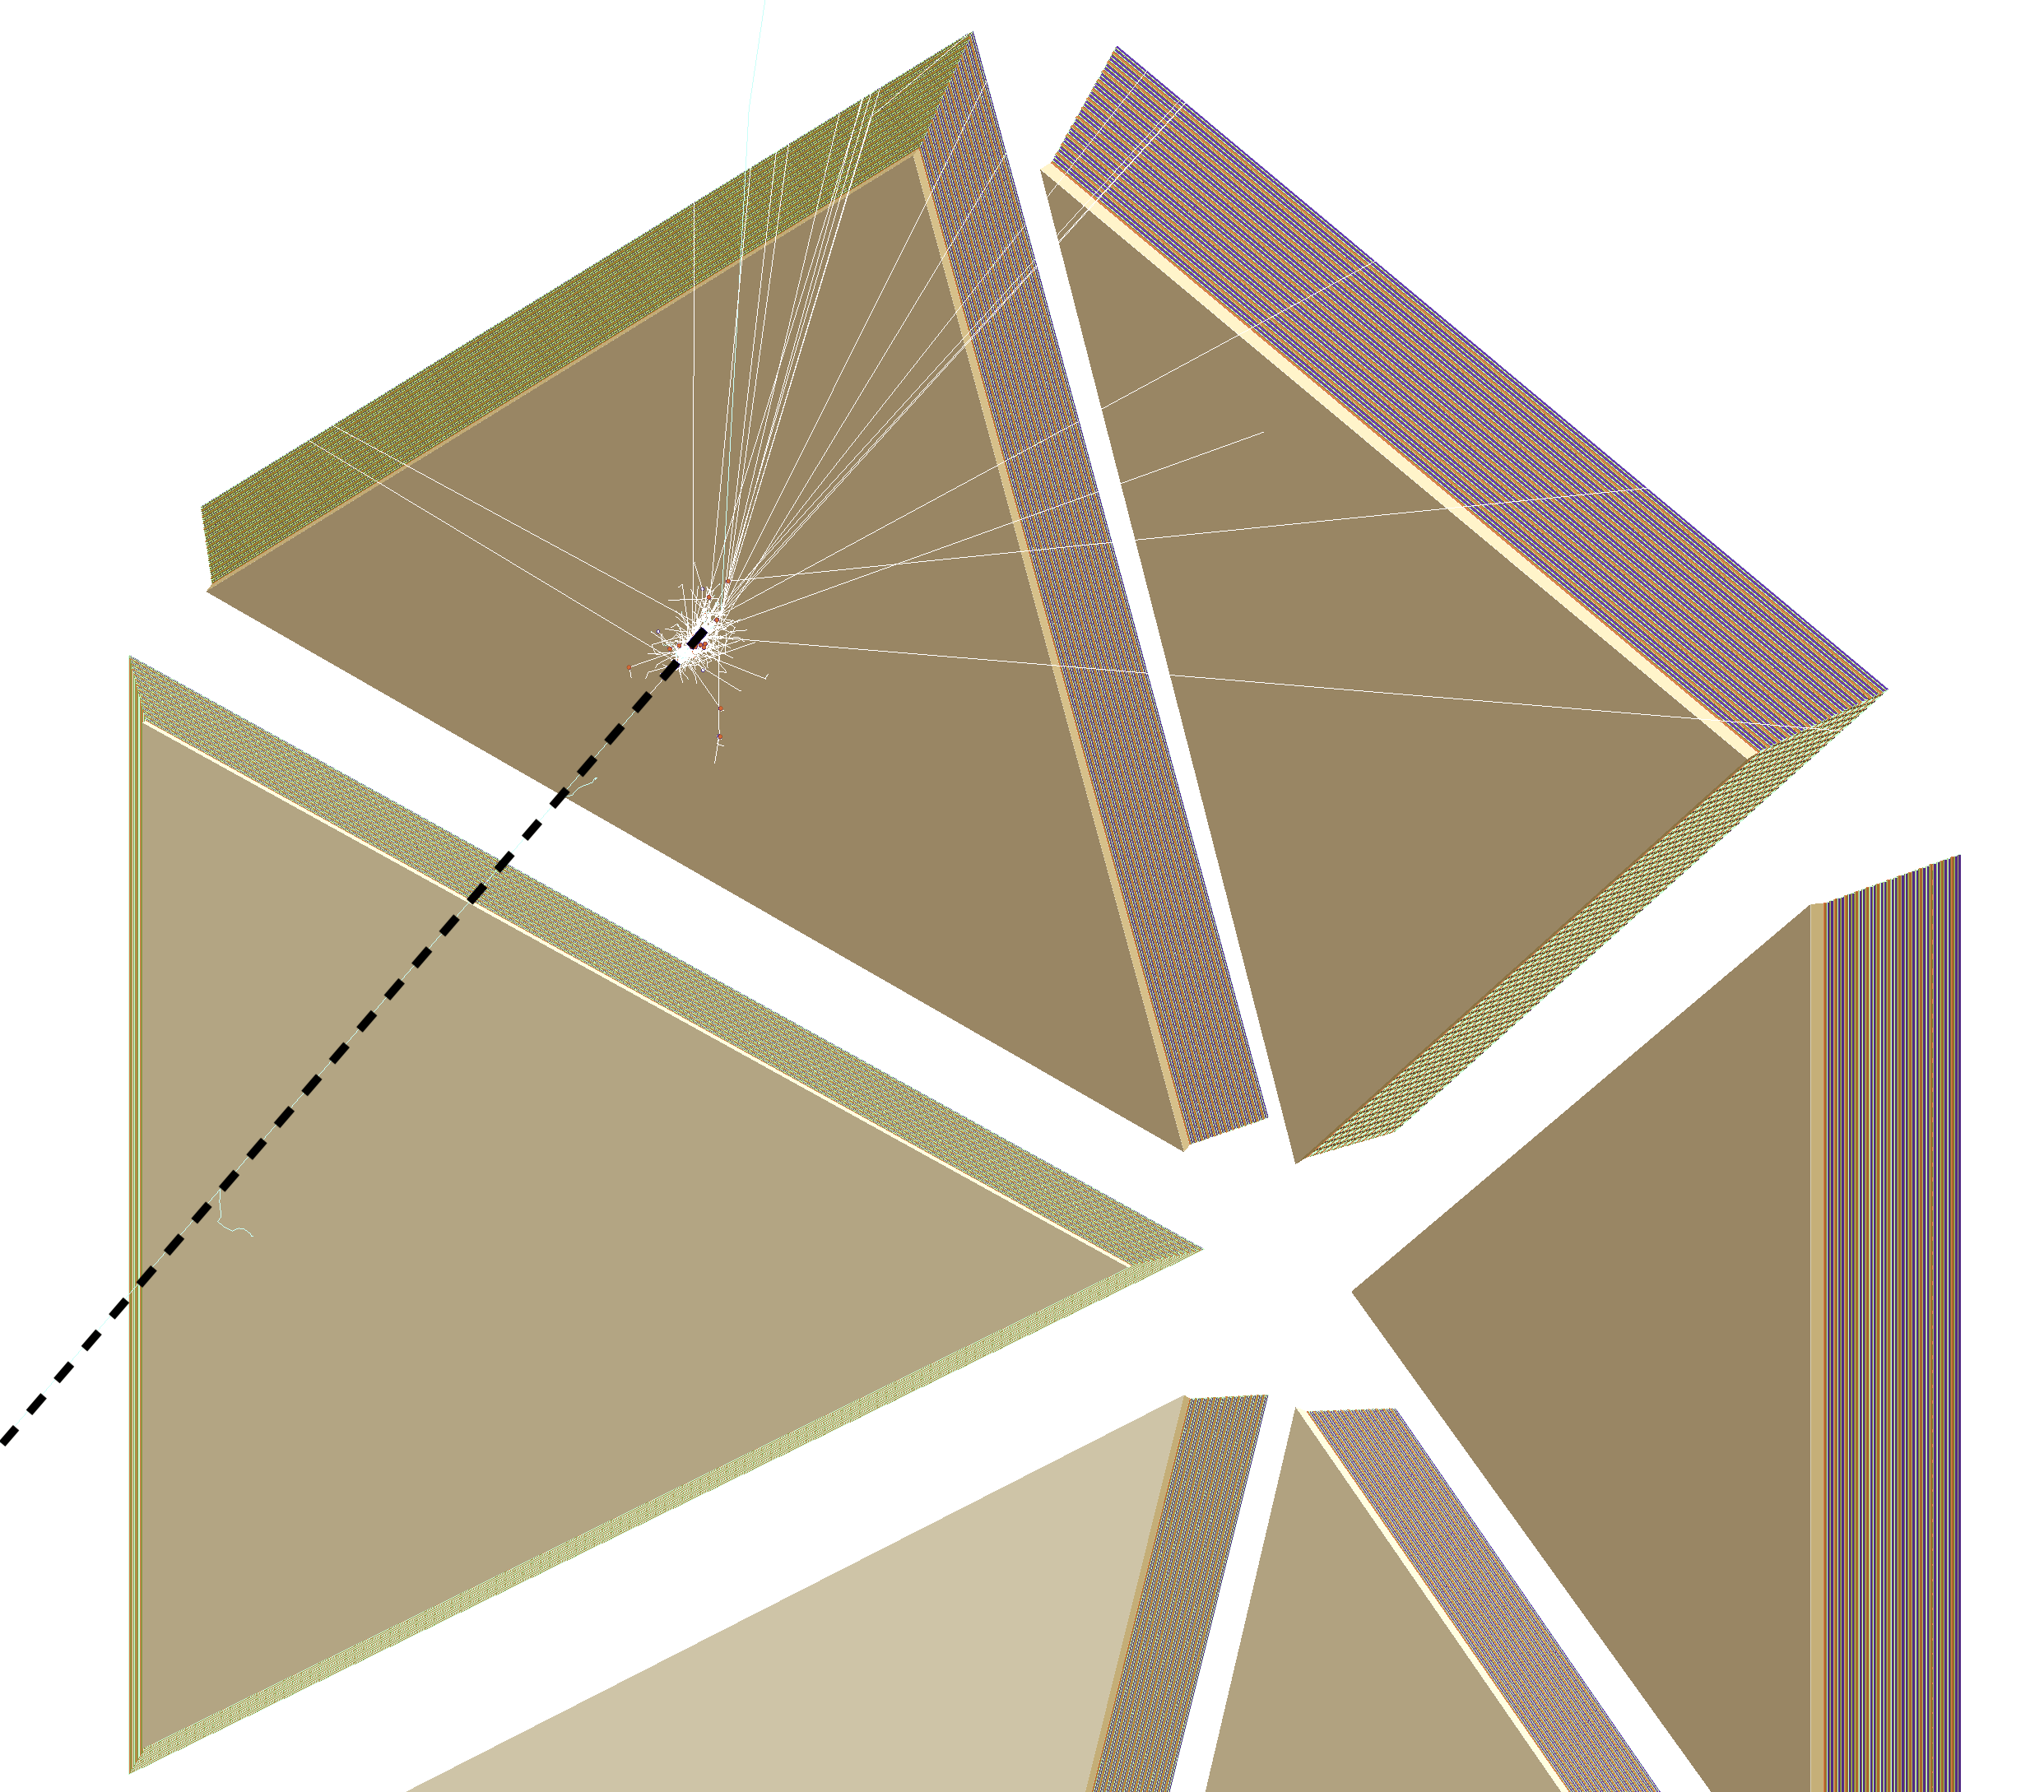
\includegraphics[width=0.99\columnwidth,keepaspectratio]{img/ecGeometry.png}
	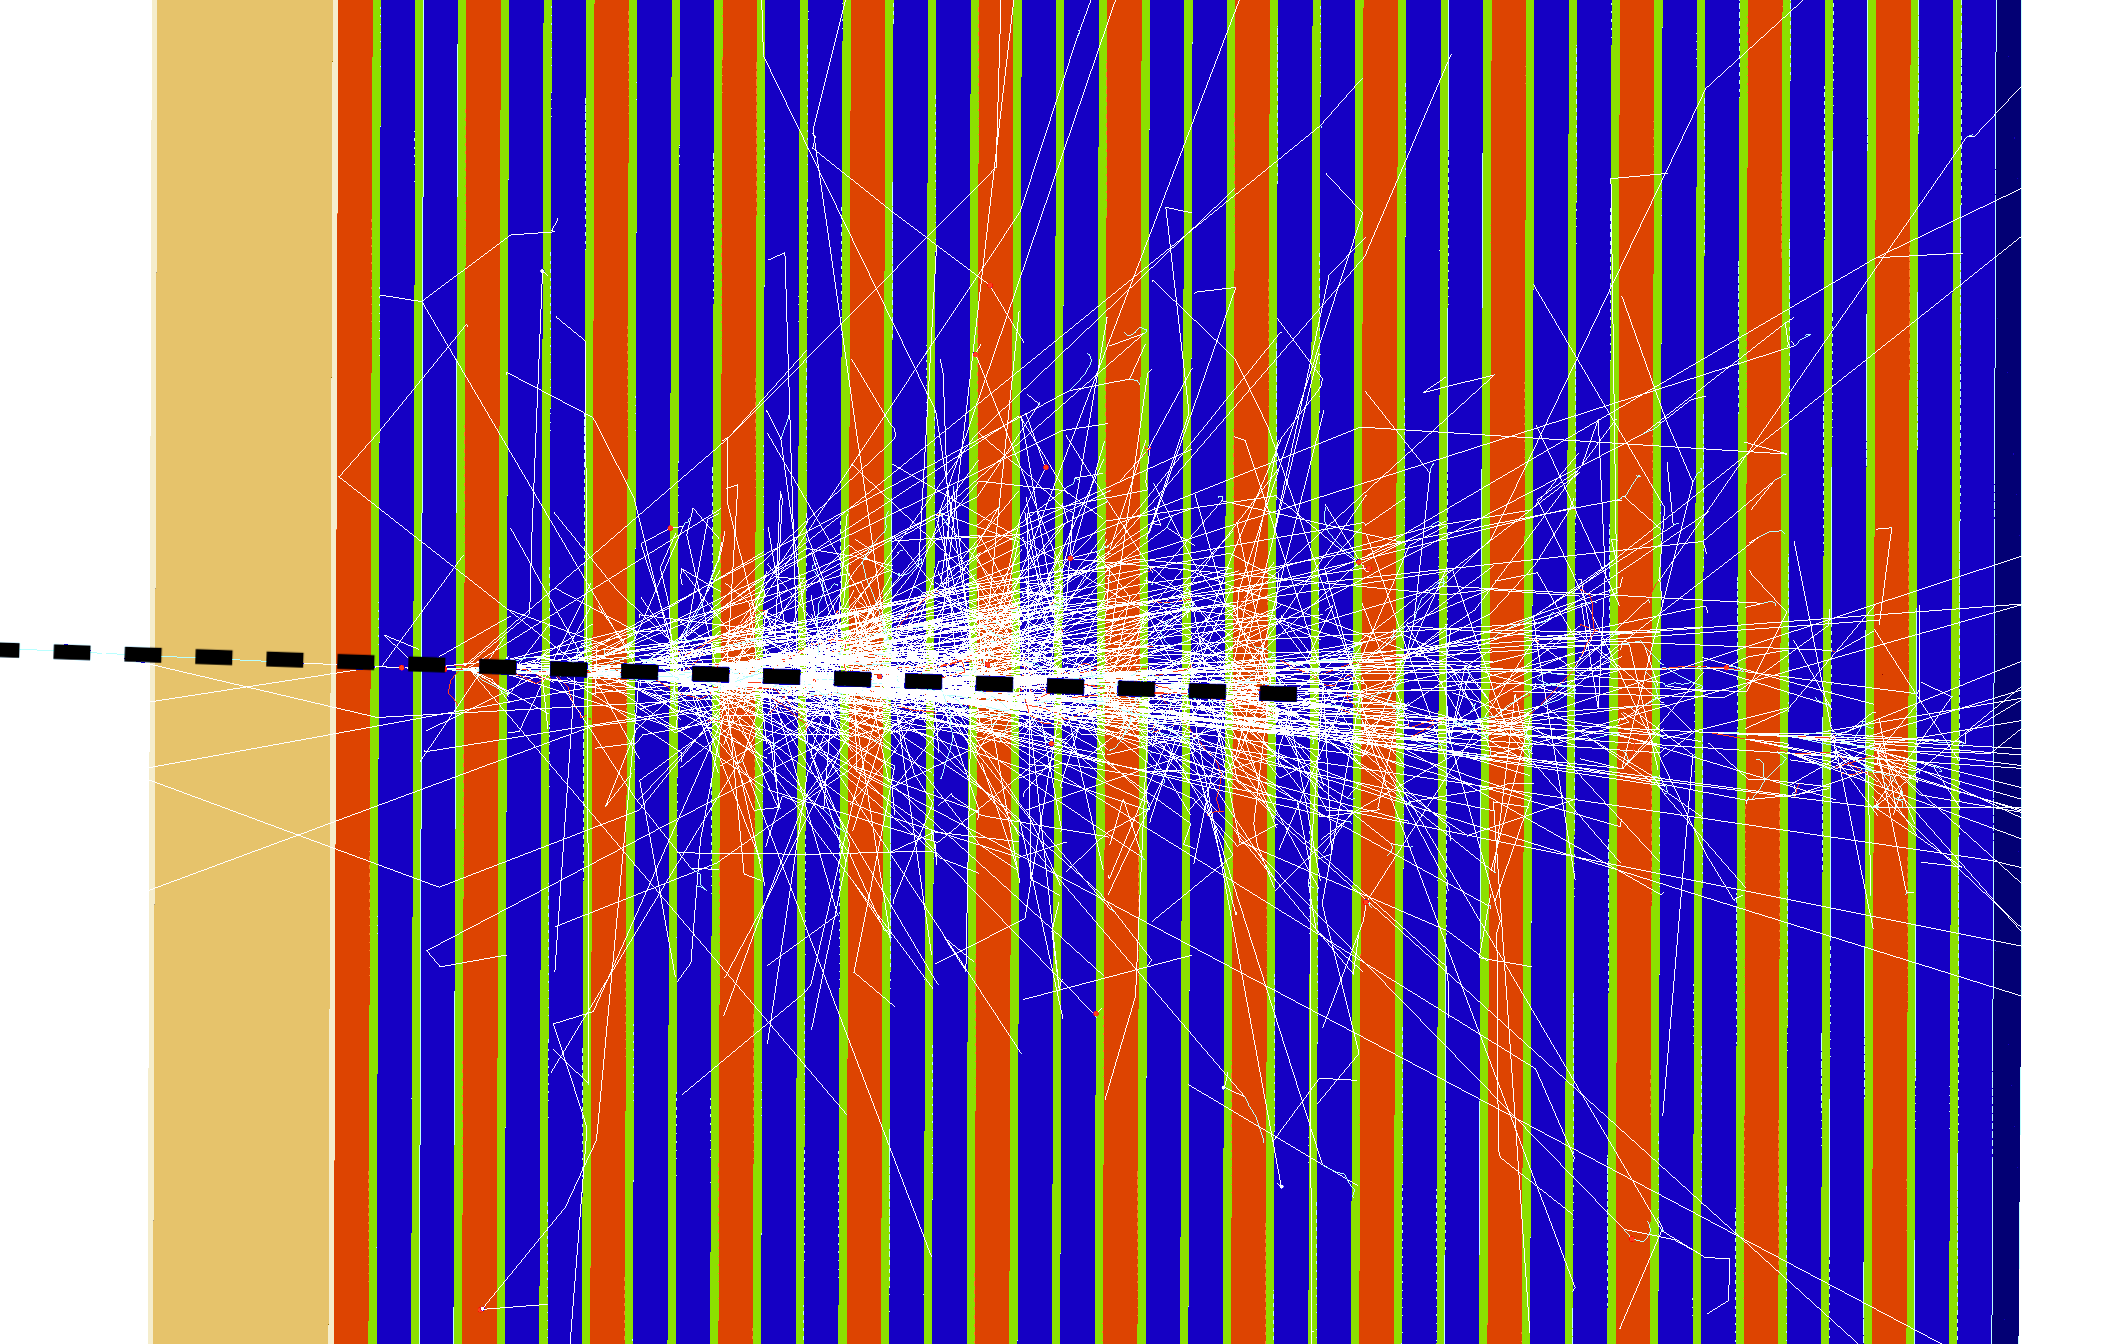
\includegraphics[width=0.99\columnwidth,keepaspectratio]{img/ecDetail.png}
	\caption{Top: a 4 GeV electron track (dotted line) showering in the GEMC implementation of the ECAL geometry.
        	 Beam is incident from the left.
             The scintillator layers alternate with a layer of lead, for a sampling fraction of about 0.3.
             Bottom: a zoom-in transverse view of the electron shower.}
	\label{fig:ecGeometry}
\end{figure}

%\begin{figure}
%	\centering
%	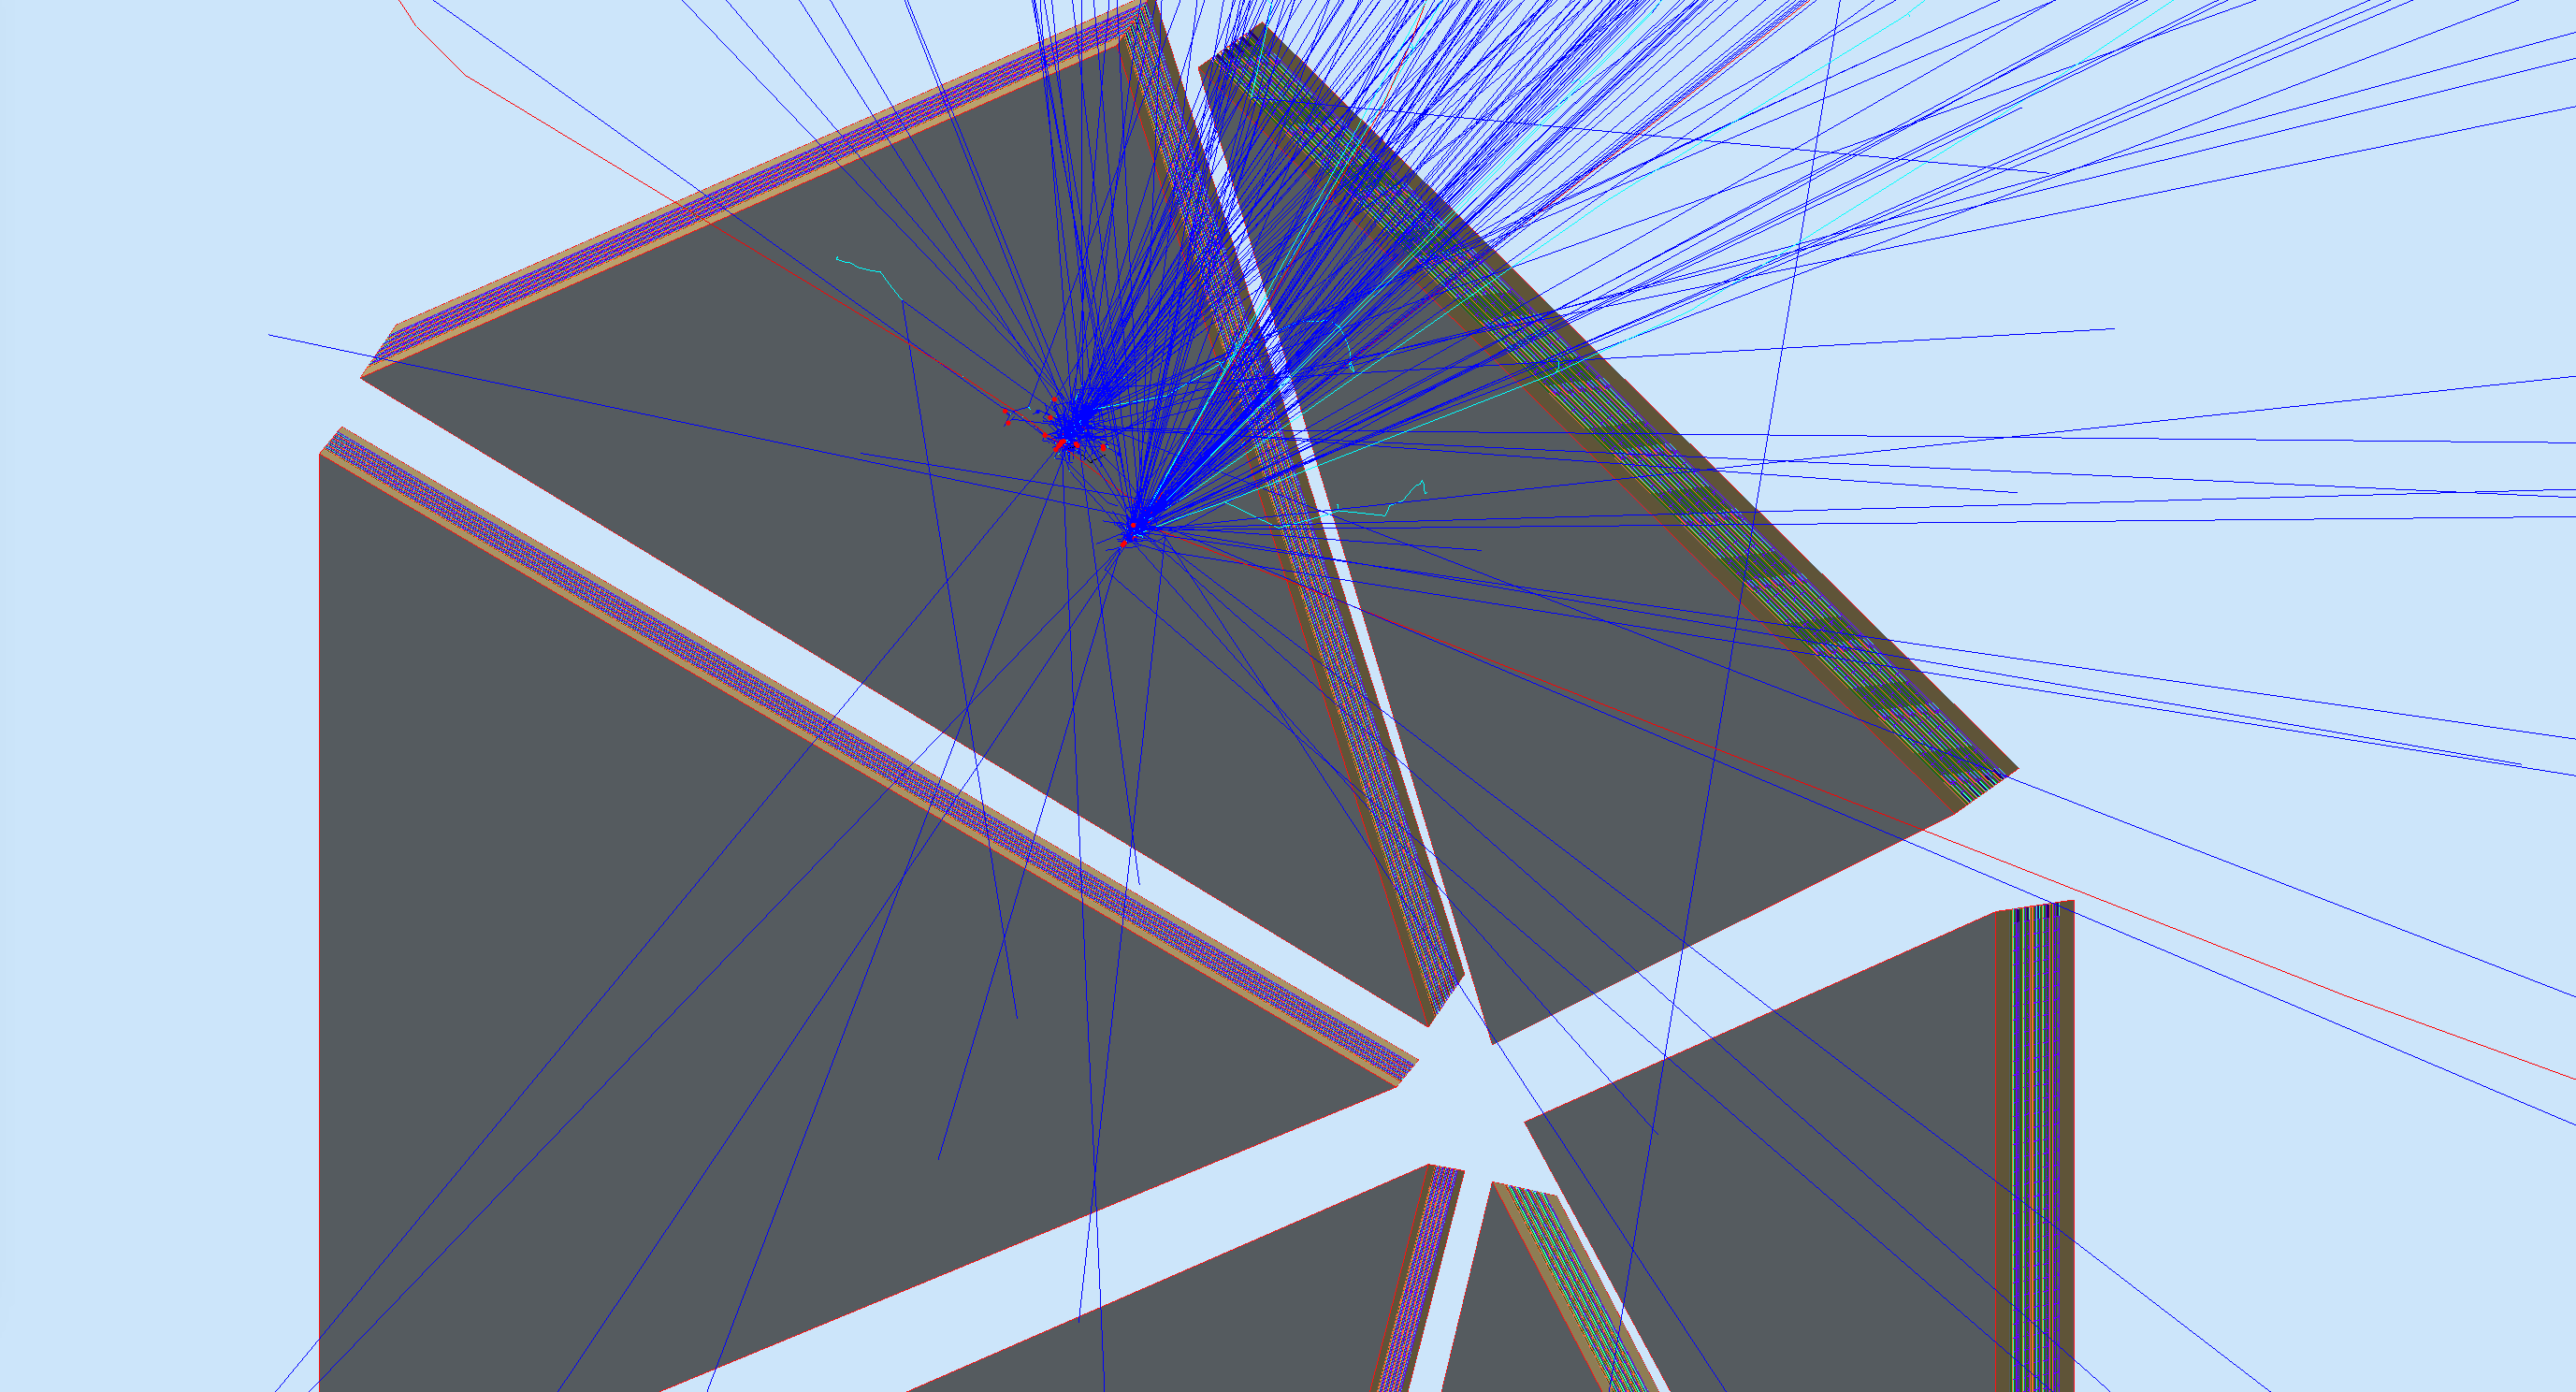
\includegraphics[width=0.99\columnwidth,keepaspectratio]{img/pcalGeometry.png}
%	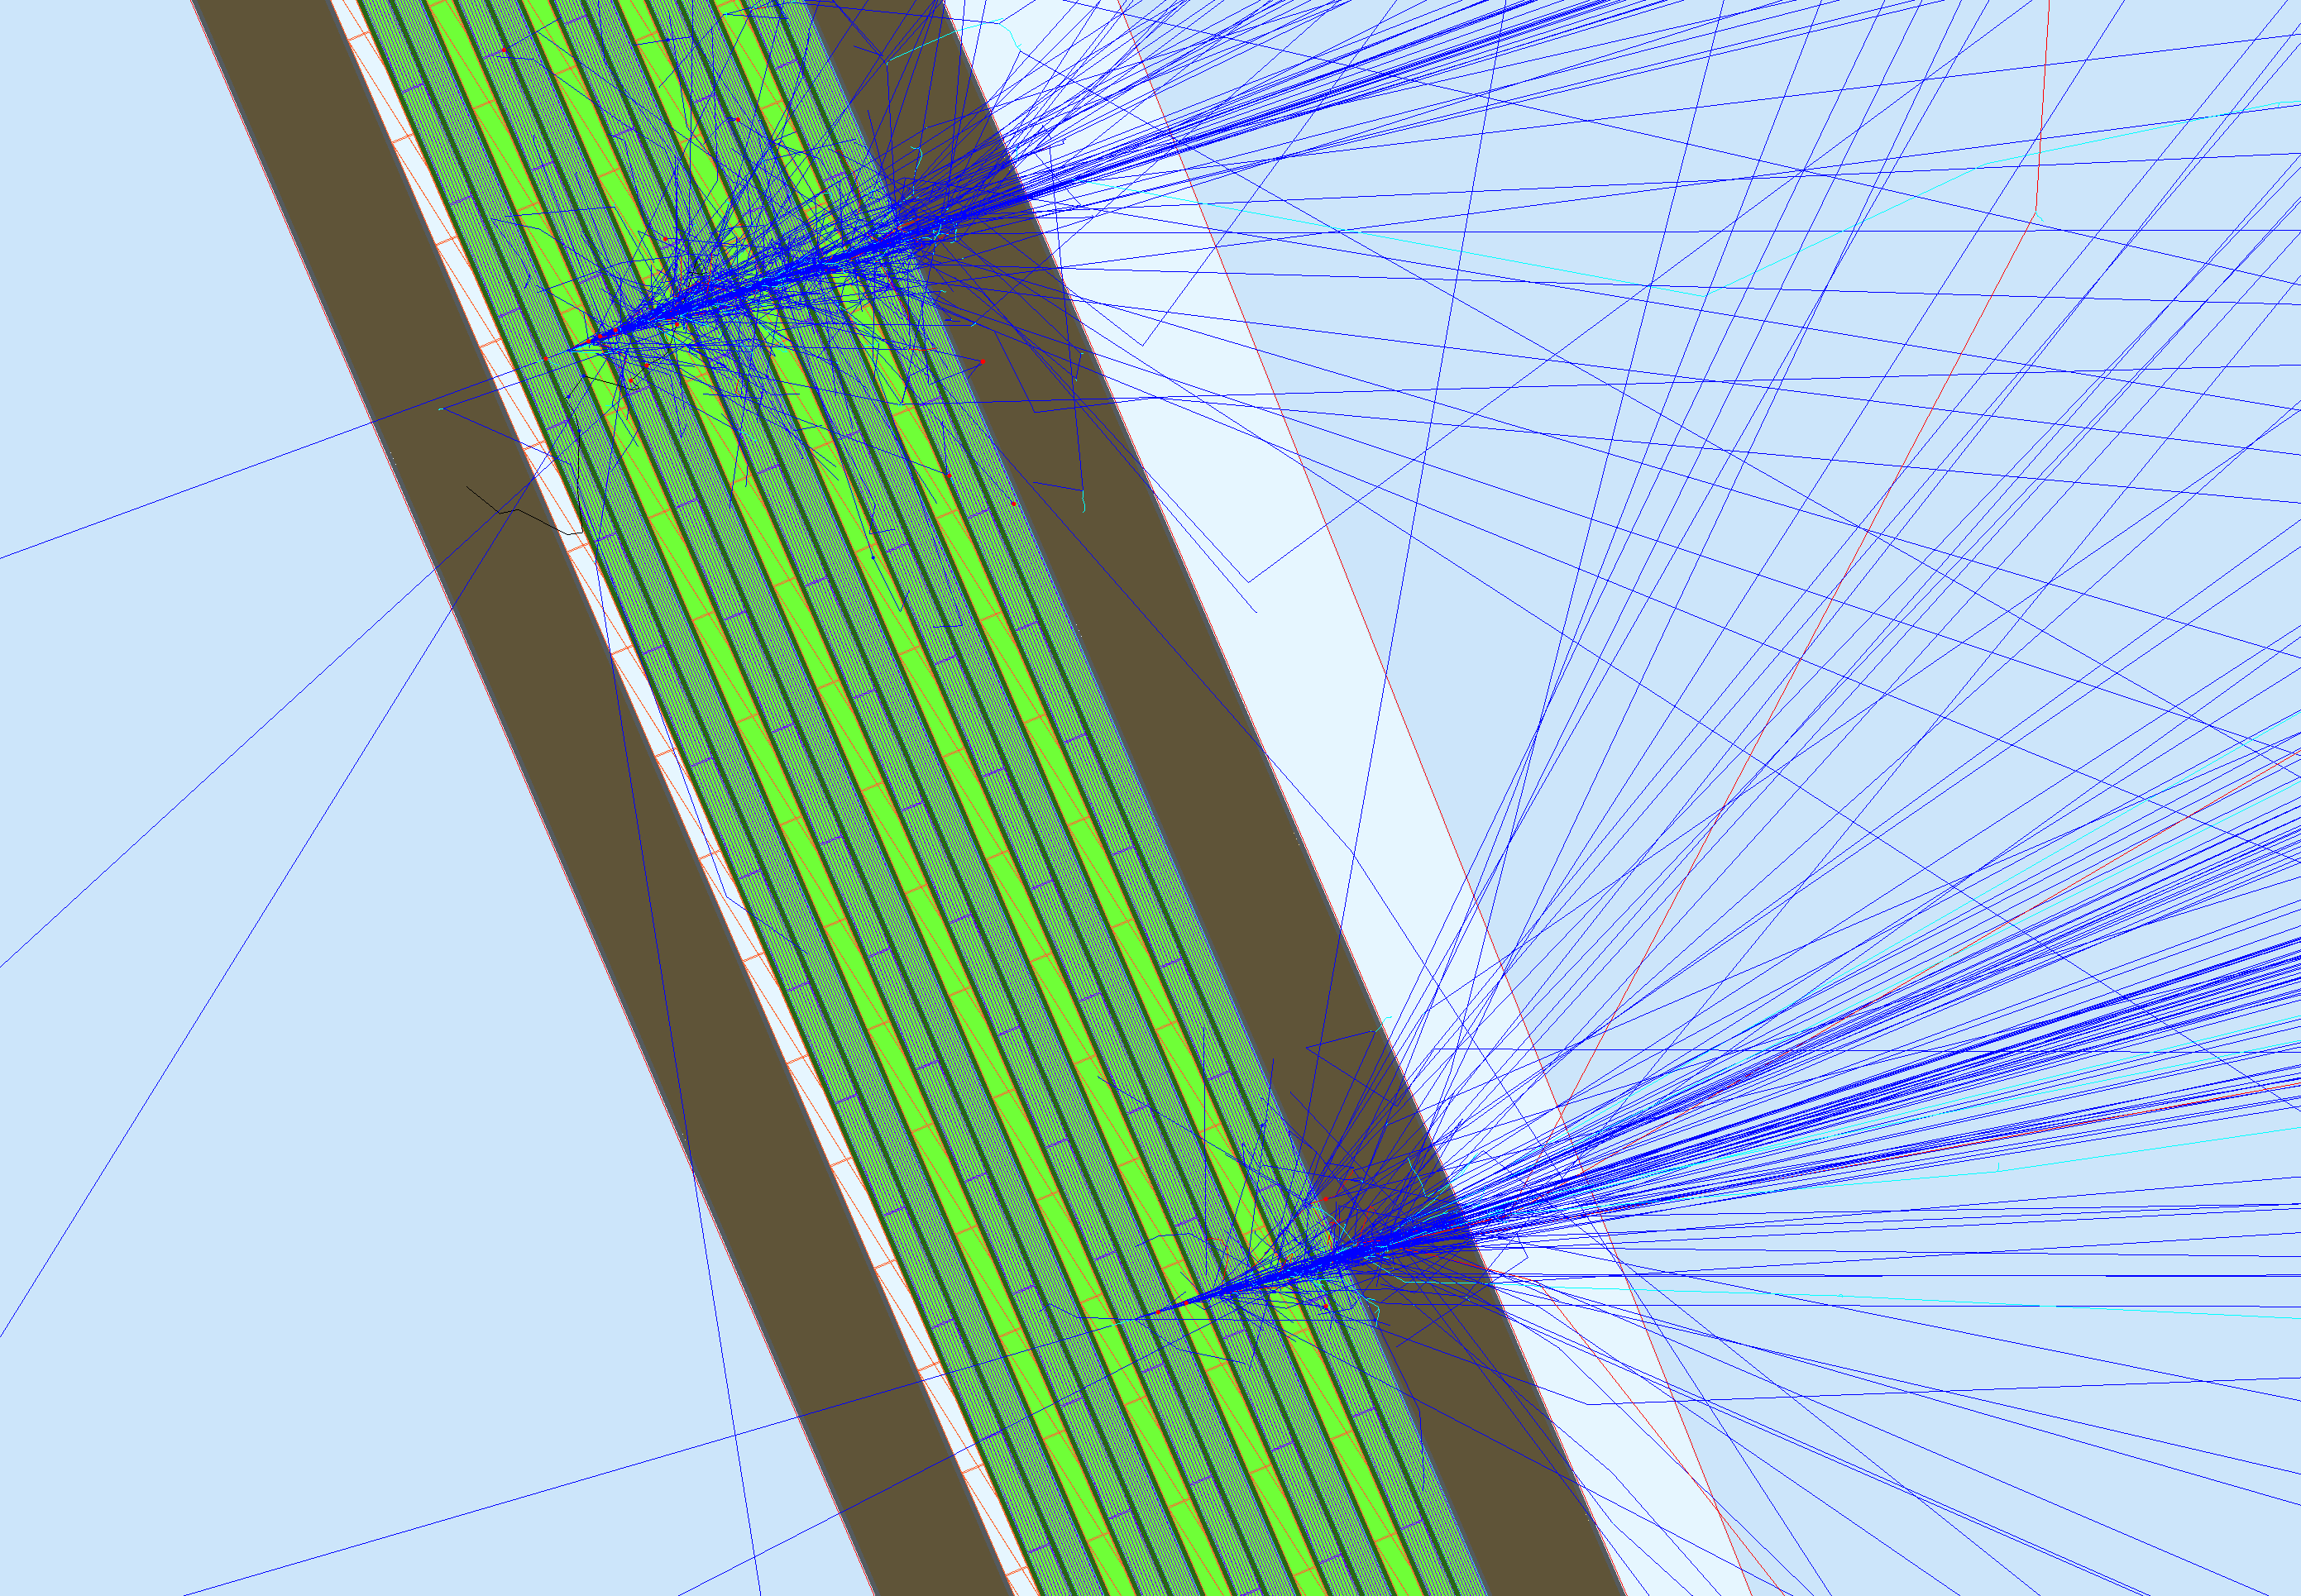
\includegraphics[width=0.99\columnwidth,keepaspectratio]{img/pcalDetail.png}
%	\caption{Top: a 4 GeV $\pi^0$ decayed in two photons hitting the GEMC implementation of the PCAL geometry.
%           The paddles are G4Boxes, embedded in trapezoid representing the mother volumes of each panel.
%            The paddles layers are alternating with trapezoid made of lead, for a sampling fraction of about 0.3.
%            Bottom: a zoom-in transverse view of showers.}
%	\label{fig:pcalGeometry}
%\end{figure}

\subsubsection{Digitization}
The digitization is the same for both the EC and the PCAL calorimeters.
The energy deposited is reduced based on the position on the scintillator using the calibrated attenuation length.
A number of photoelectrons is generated using a Poissonian distribution based on the attenuated energy.
The scintillator resolution $\sigma_{res}$ is obtained from the calibration constants, after the fluctuations in PMT gain
are taken into account using a Gaussian form with $\sigma_{res}$. A conversion factor is used to produce an ADC output.

The absolute hit time is corrected using the attenuation length and an additional factor that accounts for the time-walk correction.
The digitized output bank variables for both systems are summarized in Table \ref{tab:ecBank}.

\begin{table}[h]
	\begin{center}
		\begin{tabular}{| c | c | c |}
			\hline \hline
			Variable &                Description   \\
			\hline
             sector  &              sector number   \\
              stack  &  scintillator layer number   \\
               view  &                       view   \\
              strip  &               strip number   \\
                ADC  &                        ADC   \\
                TDC  &                        TDC   \\
               hitn  &                 hit number   \\
			\hline \hline
		\end{tabular}
	\end{center}
	\caption{The digitized EC and PCAL banks.}\label{tab:ecBank}
\end{table}


The time window of both PCAL and EC is set to 400~ns: all Geant4 steps within the same paddle and time window are collected in one hit.
